\documentclass{article}
\usepackage{ctex}
\usepackage{amsmath, amssymb, mathrsfs, amsthm}
\usepackage{booktabs}
\usepackage{geometry}
\geometry{a4paper, margin=1in}
\usepackage{titling}
\setlength{\droptitle}{30ex}
\pretitle{\begin{flushleft}\Large\bfseries}
\posttitle{\par\end{flushleft}}
\preauthor{\begin{flushleft}\fangsong}
\postauthor{\end{flushleft}}
\predate{\begin{flushleft}}
\postdate{\end{flushleft}}
\usepackage{etoolbox}
\patchcmd{\thebibliography}{\section*{\refname}}{}{}{}

\usepackage[utf8]{inputenc}
\usepackage[TS1,T1]{fontenc}
\usepackage{fourier, heuristica}
\usepackage{array, booktabs}
\usepackage{graphicx}
\usepackage[x11names]{xcolor}
\usepackage{colortbl}
\usepackage{caption}
\DeclareCaptionFont{blue}{\color{LightSteelBlue3}}

\newcommand{\foo}{\color{black}\makebox[0pt]{\textbullet}\hskip-0.5pt\vrule width 1pt\hspace{\labelsep}}

\newcommand{\upcite}[1]{\textsuperscript{\textsuperscript{\cite{#1}}}}

\usepackage{hyperref}
\hypersetup{hypertex=true,
            colorlinks=true,
            linkcolor=magenta,
            anchorcolor=magenta,
            citecolor=magenta}

\usepackage{background}
%\usepackage{amsrefs}

\newtheorem{theorem}{定理}
\newtheorem{conjecture}{猜想}
\newtheorem{corollary}{推论}
\newtheorem{lemma}{引理}
%\newtheorem{proof}{Proof}

\title{\(n^{2}+1\)的最大素因子以及关于次指数\(ABC\)猜想的改进}
\author{Hector Pasten}
\date{·Received: 27 December 2023\\·Accepted: 9 February 2024\\·Published online: 26 February 2024}

\begin{document}

\maketitle
\thispagestyle{empty}
\backgroundsetup{scale = 1, angle = 0, opacity = 0.1,
  contents = {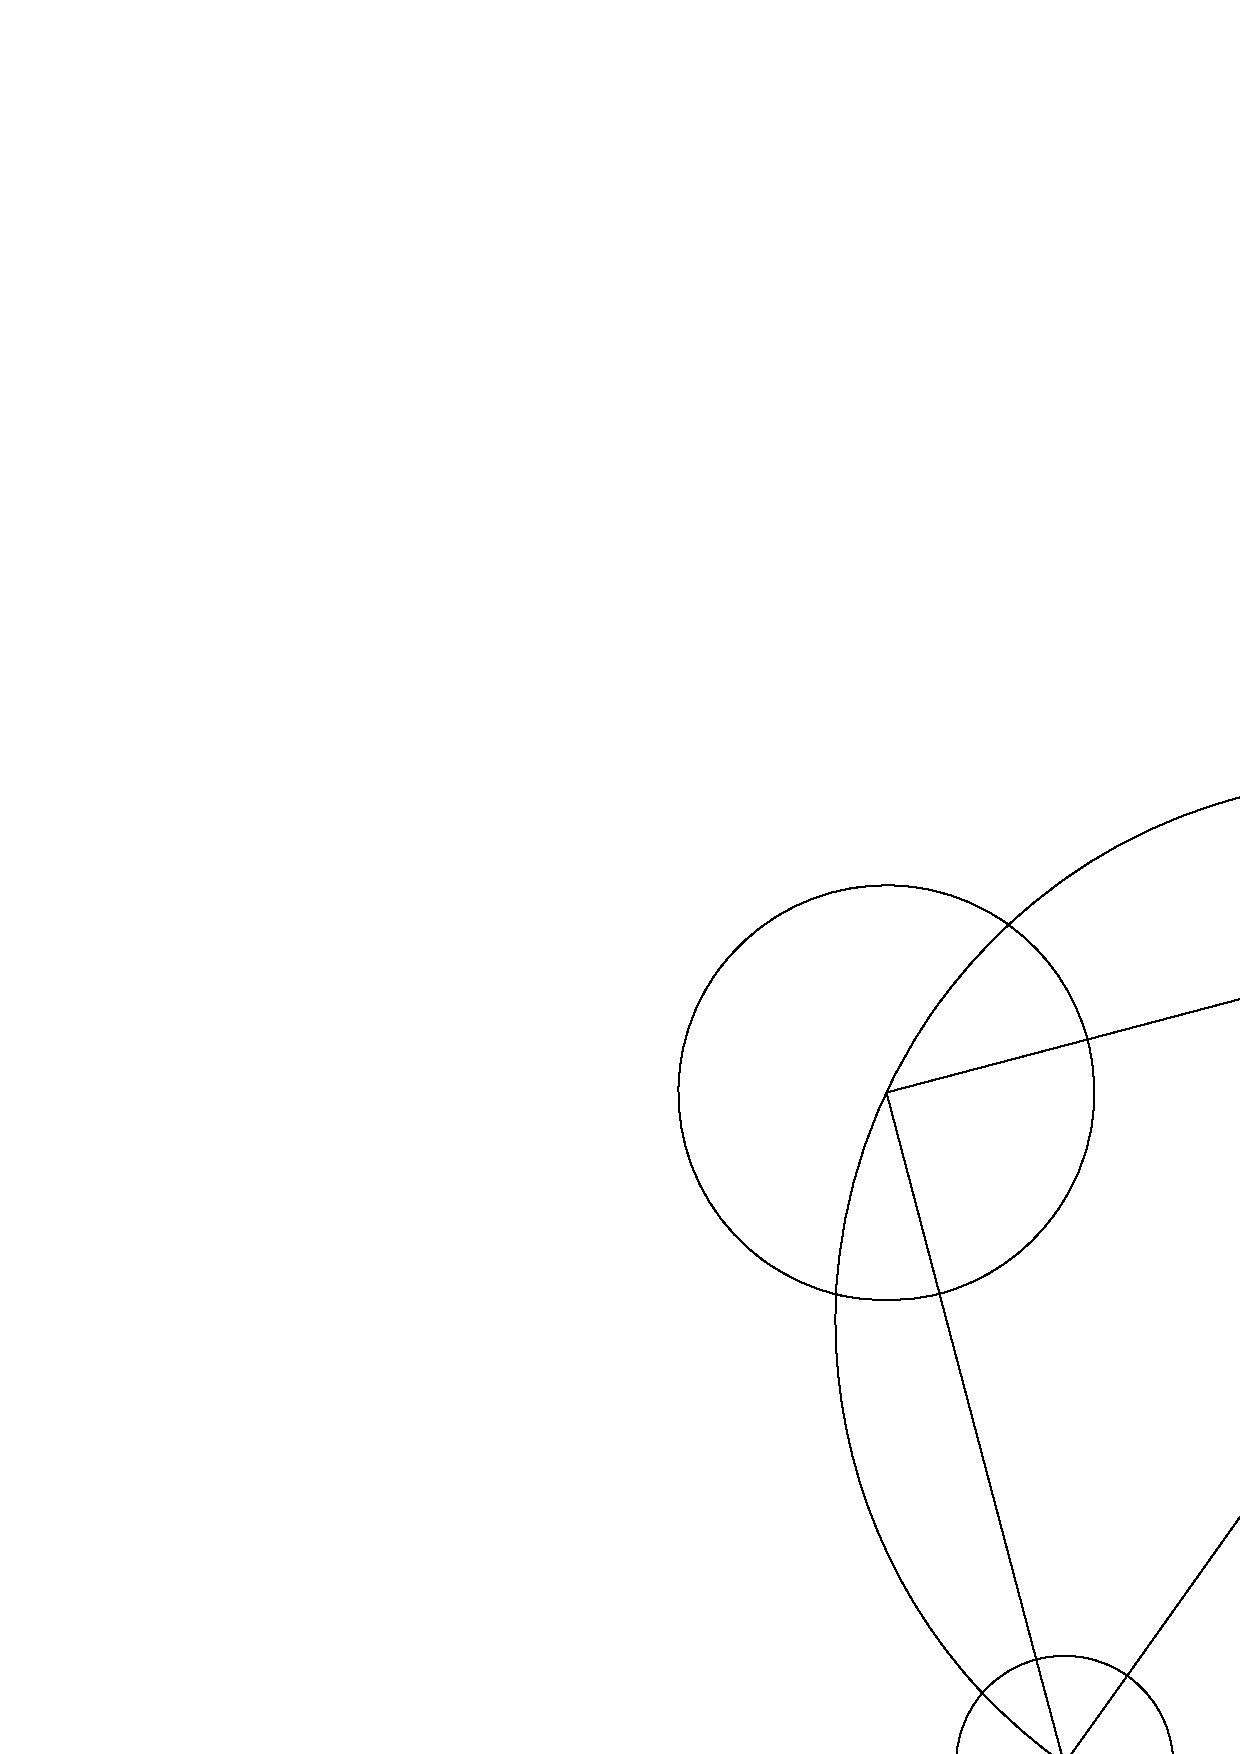
\includegraphics[width = \paperwidth,
  height = \paperheight, keepaspectratio]
  {bg.pdf}}}
  % Adjust filename and path to match your own image 
\newpage
\hrule

\part*{摘要}
\noindent
我们结合超越方法和\(ABC\)猜想的模方法,证明了\(n^{2}+1\)的最大素因子至少为\(\frac{(\log _{2}n)^{2}}{\log _{3}n}\) ,其中\(\log _{k}\)是对数函数的第\(k\)次迭代。这显著改进了现有的最佳估计,此前的估计本质上是\(\log _{2}n\)量级的,最早可追溯到1934年乔拉(Chowla)的工作。利用相同的思路,我们在\(ABC\)猜想的次指数界方面也取得了重大进展,在一种情况下,首次改进了斯图尔特(Stewart)和余(Yu)二十多年前的一个结果。我们方法的核心是作者所建立的志村曲线与\(ABC\)猜想之间的联系。

\newpage
\hrule
\part{引言}


对于非零整数\(n\),设\(\mathscr{P}(n)\)为\(n\)的最大素因子,并规定\(\mathscr{P}(\pm1)=1\)。给\(\mathscr{P}(f(n))\)确定下界是一个经典问题,其中\(f\)是整系数非线性多项式。1934年,乔拉\cite{1}证明存在正常数\(\kappa\),使得当\(n\)增大时,有
\begin{equation}
\tag{1.1}
\mathscr{P}\left(n^{2}+1\right) \geq \kappa \cdot \log _{2} n
\end{equation}
这里\(\log_{k}\)是对数函数的第\(k\)次迭代(对于迭代对数,我们总是假设自变量足够大以保证其有定义)。从那以后,这个结果被推广到所有多项式(参见\cite{9}及其中的参考文献),但90年过去了,乔拉定理仅有一些小的改进:据作者所知,目前最精确的估计是通过对数线性形式理论得到的,其形式为
\[
\mathscr{P}\left(n^{2}+1\right) \geq \kappa \cdot \frac{\log _{3} n}{\log _{4} n} \cdot \log _{2} n,
\]
见\cite{9}。我们证明了\(\mathscr{P}(n^{2}+1)\)的一个下界,几乎是之前界的平方:
\setcounter{theorem}{0} 
\renewcommand{\thetheorem}{1.\arabic{theorem}}
\begin{theorem}
存在常数\(\kappa>0\),使得当\(n\)增大时,有
\[
\mathscr{P}\left(n^{2}+1\right) \geq \kappa \cdot \frac{\left(\log _{2} n\right)^{2}}{\log _{3} n} 
\]
\end{theorem}
对于正整数\(n\),设\(\text{rad}(n)\)为其根基,即\(n\)的最大无平方因子除数。实际上,前面的结果是下一个定理的直接推论:
\begin{theorem}
存在常数\(\kappa>0\),使得当\(n\)增大时,有
\[
\text{rad}\left(n^{2}+1\right) \geq \exp \left(\kappa \cdot \frac{\left(\log _{2} n\right)^{2}}{\log _{3} n}\right) 
\]
\end{theorem}
上述定理的证明结合了对数线性形式理论,以及作者利用志村曲线理论\cite{7}发展的\(ABC\)猜想的模方法相关结果。特别地,这些方法涉及超越数论和算术几何两个领域。
更确切地说,当我们将对数线性形式应用于这个问题时,会把\(n^{2}+1\)分解式中指数较大的素数与指数较小的素数分开。然后,对于每个\(n\),我们构造一条椭圆曲线,并将\cite{7}中的结果应用于这条椭圆曲线,从而对\(n^{2}+1\)中指数较大的素因子个数给出一个较好的界。在此之后,我们利用这个新的信息,再回到对数线性形式提供的界,进而得出结论。
本文所开发的技术并不局限于前面这两个定理。事实上,我们方法的另一个应用是,能够改进\(ABC\)猜想现有的最精确次指数界。让我们回顾一下这个问题的表述。
\setcounter{theorem}{3}
\renewcommand{\theconjecture}{1.\arabic{theorem}}
\begin{conjecture}(马瑟 - 奥斯特勒\(ABC\)猜想)
设\(\epsilon>0\),存在仅依赖于\(\epsilon\)的数\(\kappa_{\epsilon}>0\),使得以下结论成立:
给定互素的正整数\(a\)、\(b\)、\(c\),且\(a + b = c\),我们有\(c \leq \kappa_{\epsilon} \cdot \text{rad}(abc)^{1+\epsilon}\) 。
\end{conjecture}
在接下来的内容中,设\(R = \text{rad}(abc)\),其中\(a\)、\(b\)、\(c\)是\(ABC\)猜想陈述中的三元组,术语“绝对常数”是指与所有参数无关的数。目前,最好的无条件界由斯图尔特 - 余\cite{12}给出,其形式为
\[
\log c \leq \kappa \cdot R^{1 / 3}(\log R)^{3}
\]
对于某个绝对常数\(\kappa\)。也可参见\cite{5,10,11}中其他的无条件界。虽然所有这些界关于\(R\)都是指数形式的,但在某些情况下可以得到更好的次指数界:

\begin{enumerate}
\item (见作者的\cite{6})设\(\epsilon>0\),存在仅依赖于\(\epsilon\)的数\(\kappa_{\epsilon}>0\),使得如果对于某个\(\eta>0\)有\(a \leq c^{1-\eta}\) ,那么
\[
\log c \leq \eta^{-1} \cdot \kappa_{\epsilon} \cdot \exp \left((1+\epsilon) \cdot \frac{\log _{3} R}{\log _{2} R} \cdot \log R\right) 
\]
\item
(见斯图尔特和余的\cite{12})设\(q = \min\{\mathscr{P}(a), \mathscr{P}(b), \mathscr{P}(c)\}\) 。那么对于某绝对常数\(\kappa>0\),我们有
\[
\log c \leq q \cdot \exp \left(\kappa \cdot \frac{\log _{3} R}{\log _{2} R} \cdot \log R\right) 
\]
\end{enumerate}
我们的方法对这两个界都有显著改进:
\begin{theorem}
设\(a\)、\(b\)、\(c\)遍历互素正整数三元组且满足\(a + b = c\),并记\(R = \text{rad}(abc)\) 。那么有以下界:
\begin{enumerate}
\item
存在绝对常数\(\kappa>0\),使得如果对于某个\(\eta>0\)有\(a \leq c^{1-\eta}\) ,那么
\[
\log c \leq \eta^{-1} \exp \left(\kappa \cdot \sqrt{(\log R) \log _{2} R}\right) 
\]
\item
设\(q = \min\{\mathscr{P}(a), \mathscr{P}(b), \mathscr{P}(c)\}\) 。存在绝对常数\(\kappa>0\),使得
\[
\log c \leq q \cdot \exp \left(\kappa \cdot \sqrt{(\log R) \log _{2} R}\right) 
\]
\end{enumerate}
\end{theorem}
值得指出的是,前面定理的第2项是二十多年来对\cite{12}中定理2的首次改进。
利用定理1.4的第2项,我们还得到了对\cite{12}中界(7)的如下改进:
\setcounter{theorem}{5}
\renewcommand{\thecorollary}{1.\arabic{theorem}}
\begin{corollary}
存在绝对常数\(\kappa>0\),使得当\(x<y\)遍历互素正整数时,我们有
\[
\mathscr{P}(xy(x + y)) \geq \kappa \cdot \frac{\left(\log _{2} y\right)^{2}}{\log _{3} y} 
\]
\end{corollary}
而\cite{12}中的界(7)为
\[
\mathscr{P}(xy(x + y)) \geq \kappa \cdot \frac{\left(\log _{2} y\right) \log _{3} y}{\log _{4} y}
\]
这反过来又是对范德波滕(van der Poorten)、辛泽尔(Schinzel)、肖里(Shorey)和蒂德曼(Tijdeman)\cite{14}早期界
\[
\mathscr{P}(xy(x + y)) \geq \kappa \cdot \log _{2} y
\]
的改进。
正如读者将看到的,通过一些整理工作,可以得到定理1.1、1.2、1.4以及推论1.5中\(\kappa\)的显式值,这些值对于足够大的变量值是有效的。我们把这个任务留给感兴趣的读者。

\newpage
\hrule
\part{预备知识}
\section{对数线性形式的界}


我们需要埃弗特斯(Evertse)和焦里(Györy)给出的关于有限生成乘法群逼近的估计(参见\cite{3}中的定理4.2.1),它来自对数线性形式理论和数的几何理论。


首先引入一些符号。设\(k\)是一个在\(\mathbb{Q}\)上次数为\(d\)的数域。如果\(v\)是\(k\)的一个阿基米德位,与嵌入\(\sigma: k \to \mathbb{C}\)相关(它可以是实嵌入,也可以是一对复共轭嵌入之一),我们在\(k\)上定义\(v -\)adic范数
\[|x|_{v}=|\sigma(x)|^{\epsilon_{v}}\]
其中\(|\cdot|\)是通常的复数绝对值,并且当\(\sigma\)是实嵌入时\(\epsilon_{v}=1\),当\(\sigma\)是复嵌入时\(\epsilon_{v}=2\)。另一方面,如果\(v\)是\(k\)的一个非阿基米德位,与\(O_{k}\)的一个素理想\(\mathfrak{p}\)相关,我们令\(v_{\mathfrak{p}}\)是\(k\)上的\(\mathfrak{p}-\)adic赋值,并定义\(v -\)adic范数
\[|x|_{v}=\text{Norm}(\mathfrak{p})^{-v_{\mathfrak{p}}(x)}\]
在\(k = \mathbb{Q}\)的情况下,当\(p\)是素数时,我们简单地用\(v_{p}\)表示\(p -\)adic赋值 。


\(k\)上的高度定义为
\[h(x)=\frac{1}{d} \sum_{v} \log \max \{1,|x|_{v}\}\]
设\(\Gamma\)是\(k^{*}\)的一个有限生成乘法子群,并且\(\{\xi_{1}, \ldots, \xi_{m}\} \subseteq \Gamma\)是\(\Gamma / \Gamma_{\text{tor}}\)的一组生成元,其中\(m \geq 1\)。在这些符号和假设下,由\cite{3}中的定理4.2.1,我们得到:
\setcounter{theorem}{0}
\renewcommand{\thetheorem}{2.\arabic{theorem}}
\begin{theorem}(逼近界)
存在仅依赖于\(d\)的数\(K_{d}\),使得以下结论成立:
\begin{enumerate}
\item
(阿基米德界)设\(v\)是\(k\)的一个阿基米德位。对于每个\(\xi \in \Gamma\)且\(\xi \neq 1\),我们有
\[- \log |1-\xi|_{v}<K_{d}^{m} \cdot (\log \max \{e, h(\xi)\}) \prod_{j = 1}^{m} h(\xi_{j})\]
\item
(非阿基米德界)设\(v\)是\(k\)的一个非阿基米德位,与\(O_{k}\)的素理想\(\mathfrak{p}\)相关。对于每个\(\xi \in \Gamma\)且\(\xi \neq 1\),我们有
\[- \log |1-\xi|_{v}<K_{d}^{m} \cdot \frac{\text{Norm}(\mathfrak{p})}{\log \text{Norm}(\mathfrak{p})}(\log \max \{e, \text{Norm}(\mathfrak{p}) h(\xi)\}) \prod_{j = 1}^{m} h(\xi_{j})\]
\end{enumerate}
\end{theorem}

\section{经典模方法对斯皮罗猜想的界}

在\cite{5}中,穆尔蒂(Murty)和作者利用经典模形式给出了斯皮罗猜想的一个无条件部分结果。
\begin{theorem}(斯皮罗型界,\cite{5})
存在绝对常数\(\kappa>0\),使得对所有定义在\(\mathbb{Q}\)上的椭圆曲线\(E\),有
\[\log \Delta \leq \kappa \cdot N \log N\]
其中\(\Delta\)和\(N\)分别是\(E\)的最小判别式和导子。
\end{theorem}
在\cite{5}中,常数\(\kappa\)被明确给出,这个结果足够强,在丢番图方程的显式计算中很有用;关于\(S -\)单位方程可参见\cite{5},其他应用可参见\cite{15}。改进内容可参见\cite{7}。


从前面的定理特别可以得到:
\setcounter{theorem}{3}
\renewcommand{\thecorollary}{2.\arabic{theorem}}
\begin{corollary}(最小判别式指数的界)
存在绝对常数\(\kappa>0\),使得对于所有定义在\(\mathbb{Q}\)上的椭圆曲线\(E\)和所有素数\(P\),有
\[v_{p}(\Delta) \leq \kappa \cdot N \log N\]
其中\(\Delta\)和\(N\)分别是\(E\)的最小判别式和导子。
\end{corollary}

\section{志村曲线的界}

在\cite{7}中,作者基于椭圆曲线的志村曲线参数化发展了一种理论,以便为\(ABC\)猜想和斯皮罗猜想获得一种新型的无条件界。下面陈述我们需要的结果。
\begin{theorem}(椭圆曲线的界,\cite{7}中的推论16.3)
设\(S\)是一个有限素数集,且\(\epsilon>0\)。存在仅依赖于\(S\)和\(\epsilon\)的数\(\kappa_{S,\epsilon}\),使得以下结论成立:
设\(E\)是定义在\(\mathbb{Q}\)上且在\(S\)之外半稳定的椭圆曲线,其最小判别式为\(\Delta\),导子为\(N\)。那么
\[\prod_{p | N^{*}} v_{p}(\Delta) \leq \kappa_{S, \epsilon} \cdot N^{11 / 2+\epsilon}\]
其中\(N^{*}\)是所有整除\(N\)但不在\(S\)中的素数的乘积。
\end{theorem}
\begin{theorem}(\(ABC\)三元组的界,\cite{7}中的定理16.8)
设\(\epsilon>0\)。存在仅依赖于\(\epsilon\)的数\(\kappa_{\epsilon}\),使得以下结论成立:
对于所有互素的正整数\(a\)、\(b\)、\(c\)且\(a + b = c\),我们有
\[\prod_{p | abc} v_{p}(abc) \leq \kappa_{\epsilon} \cdot \text{rad}(abc)^{8 / 3+\epsilon}\]
\end{theorem}
为方便读者,我们简要概述一下前面两个结果证明中的主要思路。


设\(E\)是定义在\(\mathbb{Q}\)上的椭圆曲线。根据模性定理\cite{1,13,16},存在模参数化\(\varphi: X_{0}(N) \to E\) 。通过雅克比 - 朗兰兹对应,对于每个可允许的分解\(N = DM\),存在志村曲线参数化\(\varphi_{D,M}: X_{0}^{D}(M) \to E\),特别地,\(X_{0}(N)=X_{0}^{1}(N)\)且\(\varphi=\varphi_{1,N}\) 。我们假设这些参数化具有最小次数。


起点是证明里贝特 - 高桥公式\cite{8}的一个推广,以得到公式
\[\prod_{p | D} v_{p}(\Delta)=\gamma_{D,M} \cdot \frac{\deg \varphi}{\deg \varphi_{D,M}}\]
其中有一个高度可控的误差因子\(\gamma_{D,M}\)(在最坏的情况下,对于任何\(\epsilon>0\) ,只要\(N\)足够大,就有\(h(\gamma_{D,M}) \leq (1+\epsilon) \log D\) ),这里\(\Delta\)是\(E\)的最小判别式。这个公式的重要之处在于它是全局性的:考虑了每个素数的贡献。


如果\(h(E)\)表示\(E\)的法尔廷斯高度,\(c\)是\(\varphi\)的马宁常数,那么通过\(E\)的参数化拉回\(E\)的一个奈龙微分,可以推出
\[\frac{\deg \varphi}{\deg \varphi_{D,M}}=\frac{c^{2}\| f\| ^{2} e^{2 h(E)}}{\left\| f_{D,M}\right\| _{2}^{2} e^{2 h(E)}}=\frac{c^{2}\| f\| ^{2}}{\left\| f_{D,M}\right\| _{2}^{2}}\]
其中\(\|\cdot\|_{2}\)是彼得松范数,\(f\)是与\(E\)相关联的傅里叶正规化新形式,\(f_{D,M}\)是定义在\(X_{0}^{D}(M)\)的整模型上的四元数模形式,它是与\(f\)相关的雅克比 - 朗兰兹对应形式。


工作的一个重要部分是证明马宁常数\(c\)的一致上界(固定加法约化的素数集)。另一方面,已知\(\|f\|_{2}^{2} \ll_{\epsilon} N^{1+\epsilon}\) \cite{4}。由于\(f_{D,M}\)可以延拓到\(X_{0}^{D}(M)\)的整模型上,所以可以使用阿拉克洛夫理论给出\(\left\|f_{D,M}\right\|_{2}^{2} \gg_{\epsilon} N^{-(5 / 3+\epsilon)} M^{-1}\)的多项式下界。为此,至关重要的是根据\(L\)函数得到黑格纳点的阿拉克洛夫高度的界(这是袁 - 张在科尔梅兹猜想背景下对乔拉 - 塞尔伯格公式的推广\cite{17}),以及相关\(L\)函数合适的无零点区域。将所有这些结合起来,最终得到
\[\prod_{p | D} v_{p}(\Delta) \ll_{\epsilon} N^{8 / 3+\epsilon} D M=N^{11 / 3+\epsilon}\]
通过改变\(M\)的选择得到定理2.4。通过选择\(E\)为弗雷 - 赫勒高奇椭圆曲线得到定理2.5,在这种情况下可以证明更强的界\(h(\gamma_{D,M}) \leq \epsilon \log D\) 。

\newpage
\hrule
\part{\(n^{2}+1\)的最大素因子}

下面这个简单的观察结果会被多次用到。

\setcounter{lemma}{0}
\renewcommand{\thelemma}{3.\arabic{lemma}}
\begin{lemma}
考虑一个数\(A>e\) 。实函数\(t \mapsto t \log (A / t)\)在\(1 \leq t \leq A / e\)这个区间内是单调递增的。
\end{lemma}


下一个引理给出的界并非该方法所能得到的最佳界,但对我们的目的来说已经足够。
\begin{lemma}
存在一个绝对常数\(K>0\),使得对于所有正整数\(n\),我们有
\[
\prod_{p | n^{2}+1} v_{p}\left(n^{2}+1\right) \leq K \cdot \text{rad}\left(n^{2}+1\right)^{8} 
\]
\end{lemma}
\begin{proof}
设\(n\)是一个正整数,考虑椭圆曲线
\[
E: y^{2}=x^{3}+3 x + 2n
\]
设\(\Delta\)和\(N\)分别是\(E\)的最小判别式和导子。这个魏尔斯特拉斯方程除了可能在\(2\)和\(3\)处之外都是极小的,并且它有(不一定是最小的)判别式
\[
-16\left(4 \cdot 3^{3}+27(2n)^{2}\right)=-1728\left(n^{2}+1\right)
\]
可以验证\(E\)在\(2\)和\(3\)之外有乘法约化(因此,除了\(2\)和\(3\)的有界次幂之外,\(N\)是无平方因子的),并且最小判别式是
\[
\Delta=-2^{s} \cdot 3^{t} \cdot\left(n^{2}+1\right)
\]
其中\(s\)和\(t\)是绝对值有界的整数。


根据推论2.3,存在一个绝对常数\(\kappa>0\),使得
\[
v_{2}\left(n^{2}+1\right) v_{3}\left(n^{2}+1\right) \leq \kappa \cdot N^{2}(\log N)^{2} 
\]
令\(\epsilon>0\),并选择\(S = \{2,3\}\),应用定理2.4,我们得到一个仅依赖于\(S\)和\(\epsilon\)的数\(\kappa_{S,\epsilon}\),使得
\[
\prod_{p | N^{*}} v_{p}\left(n^{2}+1\right) \leq \kappa_{S, \epsilon} \cdot N^{11 / 2+\epsilon}
\]
其中\(N^{*}\)是除了\(2\)和\(3\)之外整除\(N\)的素数的乘积。对于\(p\neq2,3\)的素数,\(p\)整除\(N\)当且仅当它整除\(\Delta\),进而当且仅当它整除\(n^{2}+1\) 。由此可得
\[
\prod_{p | n^{2}+1} v_{p}\left(n^{2}+1\right) \leq \kappa \cdot \kappa_{S, \epsilon} \cdot N^{15 / 2+\epsilon} 
\]
因为\(S\)是固定的,我们可以选择\(\epsilon = 1/2\),从而得到
\[
\prod_{p | n^{2}+1} v_{p}\left(n^{2}+1\right) \leq K \cdot \text{rad}\left(n^{2}+1\right)^{8}
\]
对于某个绝对常数\(K>0\),这是因为\(\text{rad}(n^{2}+1)\)和\(N\)除了可能相差\(2\)和\(3\)的有界次幂之外是一致的(这是由于在\(p\neq2,3\)的素数处的半稳定约化)。
\end{proof}

\begin{proof}[定理1.2的证明]
设\(n\)是一个足够大的正整数,并且记\(i = \sqrt{-1} \in \mathbb{C}\) 。我们考虑\(\mathbb{Z}[i]\)中的方程
\[
(n + i)-(n - i)=2i
\]
这给出了在二次数域\(k = \mathbb{Q}(i)\)中的方程
\[
1-\frac{n - i}{n + i}=\frac{2i}{n + i}
\]

考虑\(n + i = u \cdot \gamma_{1}^{e_{1}} \cdots \gamma_{r}^{e_{r}}\)的分解,其中\(\gamma_{j}\)是\(\mathbb{Z}[i]\)中互不相伴的不可约元素,\(u \in \{ \pm 1, \pm i\}\) 。那么我们有\(n - i=\overline{u} \cdot \overline{\gamma}_{1}^{e_{1}} \cdots \overline{\gamma}_{r}^{e_{r}}\),这里上划线表示复共轭。

设
\[
B=\exp \left(\sqrt{(\log R) \log _{2} R}\right)
\]
其中\(R=\text{rad}(n^{2}+1)\) 。在接下来的内容中,我们将使用\(R\)随着\(n\)增大而增大这个事实(例如,根据乔拉的结果),尽管我们不需要精确的增长速率。

定义\(J = \{1, \ldots, r\}\),并且设\(I \subseteq J\)是满足\(e_{j}>B\)的指标集。设\(\xi_{j}=\overline{\gamma}_{j} / \gamma_{j}\)对于\(j \in J\),并且设\(\xi_{0}=\prod_{j \in J - I} \xi_{j}^{e_{j}}\) 。设\(w=\overline{u} / u\) 。那么我们有
\[
\frac{n - i}{n + i}=w \cdot \xi_{0} \cdot \prod_{j \in I} \xi_{j}^{e_{j}}
\]
设\(I_{0}=I \cup \{0\}\),并且设\(\Gamma\)是由\(w\)和\(j \in I_{0}\)的\(\xi_{j}\)生成的\(k^{\times}\)的子群。设\(m = 1+\#I=\#I_{0}\) 。那么\(j \in I_{0}\)的\(\xi_{j}\)生成\(\Gamma / \Gamma_{\text{tor}}\),并且我们可以写成
\[
\frac{2i}{n + i}=1-\xi
\]
其中\(\frac{n - i}{n + i}=\xi=w \cdot \xi_{0} \cdot \prod_{j \in I} \xi_{j}^{e_{j}} \in \Gamma\) 。定理2.1的第1项(取\(d = 2\) )给出一个绝对常数\(K\),使得
\[
\log n \leq -2 \log \frac{2}{|n + i|}=-\log |1-\xi|^{2} \leq K^{m} \cdot (\log \max \{e, h(\xi)\}) \prod_{j \in I_{0}} h(\xi_{j}) \tag{3.1}
\]
其中\(|\cdot|\)是\(\mathbb{C}\)上通常的绝对值。我们来估计(3.1)右边的项。首先我们有
\[
h(\xi)=h\left(\frac{n - i}{n + i}\right) \leq \frac{1}{2} \log |n + i|^{2}=\log |n + i|
\]
所以
\[
K^{m} \cdot (\log \max \{e, h(\xi)\}) \leq (2K)^{m} \log _{2} n. \tag{3.2}
\]
另一方面,对于每个\(j \in J - I\)有\(e_{j} \leq B\),并且由于\(\gamma_{j}\)是互不相伴的不可约元素,我们得到
\[
h(\xi_{0}) \leq B \cdot h\left(\prod_{j \in J - I} \gamma_{j}\right) \leq \frac{B}{2} \log \prod_{j \in J} \text{Norm}(\gamma_{j}) \leq B \log \prod_{p | n^{2}+1} p
\]
这就给出
\[
h(\xi_{0}) \leq B \cdot \log R. \tag{3.3}
\]
此时我们注意到,如果\(m = 1\)(即\(I = \varnothing\) ),那么由(3.1)、(3.2)和(3.3)可得
\[
\sqrt{\log n} \leq \frac{\log n}{\log _{2} n} \leq 2K B \log R<\exp \left(K' \cdot \sqrt{(\log R) \log _{2} R}\right)
\]
对于一个合适的绝对常数\(K'>0\),此时结论得证。所以我们可以假设\(m \geq 2\) 。

设\(p_{j}\)是\(\gamma_{j}\)下方的素数。注意到对于\(j \in I\),我们有\(h(\xi_{j}) \leq \log p_{j}\),所以
\[
\prod_{j \in I} h(\xi_{j}) \leq \prod_{j \in I} \log p_{j} \leq \left(\frac{\log R}{m - 1}\right)^{m - 1}
\]
这里我们使用了算术 - 几何平均不等式。将其与(3.1)、(3.2)和(3.3)结合起来,我们推断出
\[
\begin{aligned} 
\sqrt{\log n} & \leq \frac{\log n}{\log _{2} n} \leq (2K)^{m} B(\log R)\left(\frac{\log R}{m - 1}\right)^{m - 1} \\ 
& =2K B(\log R)\left(\frac{2K \cdot \log R}{m - 1}\right)^{m - 1} 
\end{aligned}
\]
接下来,我们注意到
\[
e_{j}=v_{(\gamma_{j})}(n + i) \leq 2 v_{p_{j}}\left(n^{2}+1\right)
\]
因此\(e_{j}>B\)这个条件意味着\(v_{p_{j}}(n^{2}+1)>B / 2\),满足前一个条件的指标\(j\)的个数是\(m - 1=\#I\) 。这就给出
\[
\prod_{j \in I} v_{p_{j}}\left(n^{2}+1\right)>(B / 2)^{m - 1}
\]
另一方面,根据引理3.2,我们有
\[
\prod_{p | n^{2}+1} v_{p}\left(n^{2}+1\right) \leq \kappa \cdot R^{8}
\]
对于某个绝对常数\(\kappa\)。由此可得
\[
m - 1<\frac{8 \log R+\log \kappa}{\log (B / 2)}<\kappa' \cdot \frac{\log R}{\sqrt{(\log R) \log _{2} R}}=\kappa' \cdot \sqrt{\frac{\log R}{\log _{2} R}}
\]
对于一个合适的绝对常数\(\kappa'\) 。

使用引理3.1,取\(A = 2K \log R\),并且由于对于足够大的\(R\)有
\[
\kappa' \cdot \sqrt{\frac{\log R}{\log _{2} R}}<\frac{2K}{e} \log R
\]
我们推断出
\[
\begin{aligned} 
\left(\frac{2K \cdot \log R}{m - 1}\right)^{m - 1} & \leq \left(\frac{2K}{\kappa'} \sqrt{(\log R) \log _{2} R}\right)^{\kappa' \sqrt{(\log R) / \log _{2} R}} \\ 
& \leq \exp \left(K'' \cdot \sqrt{(\log R) \log _{2} R}\right) 
\end{aligned}
\]
对于一个合适的绝对常数\(K''\) 。将其代入(3.4),我们得到
\[
\sqrt{\log n} \leq 2K B(\log R) B^{K''} 
\]
因此,对于一个合适的绝对常数\(M>0\),我们得到
\[
\log n \leq \exp \left(M \cdot \sqrt{(\log R) \log _{2} R}\right)
\]
结论得证。
\end{proof}

\begin{proof}[定理1.1的证明]
记\(R=\text{rad}(n^{2}+1)\) 。根据定理1.2,我们有
\[
R \geq \exp \left(\kappa \cdot \frac{\left(\log _{2} n\right)^{2}}{\log _{3} n}\right)
\]
记\(P=\mathscr{P}(n^{2}+1)\) 。根据\(\theta(x)=\sum_{p \leq x} \log p\)的切比雪夫界,我们有
\[
R \leq \prod_{p \leq P} p \leq \exp (4P)
\]
由此结论得证。
\end{proof}

\newpage
\hrule
\part{次指数\(ABC\)猜想,情形1}
\begin{proof}[定理1.4第1项的证明]
我们保持陈述中的符号,并且假设\(c\)足够大。注意到\(R\)随着\(c\)增大而增大(例如,根据\(S -\)单位方程解的有限性)。我们可以写成
\[\frac{a}{c}=1 - \xi\]
其中\(\xi = \frac{b}{c}\)。设\(\xi_{1}, \ldots, \xi_{r}\)是\(bc\)不同的素因子,并且设\(e_{j} = v_{\xi_{j}}(b / c)\)(可能为负)。设
\[B = \exp\left(\sqrt{(\log R)\log_{2}R}\right)\]
并且定义\(J = \{1, 2, \ldots, r\}\)和\(I = \{j \in J: |e_{j}| > B\}\)。设\(\xi_{0} = \prod_{j \in J - I}\xi_{j}^{e_{j}}\),设\(I_{0} = I \cup \{0\}\),并且设\(m = \#I_{0}\)。设\(\Gamma\)是由\(j \in I_{0}\)的\(\xi_{j}\)生成的\(\mathbb{Q}^{\times}\)的子群;特别地,\(\xi = \frac{b}{c} \in \Gamma\)。

根据定理2.1的第1项,我们有
\[\eta \cdot \log c \leq \log(c / a)= - \log|1 - \xi| \leq K^{m} \cdot (\log\max\{e, h(\xi)\})\prod_{j \in I_{0}}h(\xi_{j})\]
其中\(|\cdot|\)是\(\mathbb{Q}\)上的阿基米德绝对值,\(K\)是一个绝对常数。

我们有\(h(\xi)=h(b / c)=\log c \leq R^{K'}\),对于某个绝对常数\(K'\)(例如利用\cite{10}中给出的\(ABC\)猜想的指数界,可得\(K' = 15\) )。另一方面,我们有\(h(\xi_{0})\leq B\log R\),所以我们得到
\[\eta\cdot\log c\leq K'\cdot K^{m}B(\log R)^{2}\prod_{j\in I}h(\xi_{j})\tag{4.1}\]
如果\(m = 1\),我们有\(I=\varnothing\),从而得到
\[\eta\cdot\log c\leq K'KB(\log R)^{2}\leq\exp\left(2\sqrt{(\log R)\log_{2}R}\right)\]
结果得证。所以我们可以假设\(m\geq2\)。由(4.1)式我们得到
\begin{flalign}
\tag{4.2}
\eta\cdot\log c&\leq K'\cdot K^{m}B(\log R)^{2}\left(\frac{1}{m - 1}\log R\right)^{m - 1}\\ \notag
&\leq K'KB^{2}\left(\frac{K}{m - 1}\log R\right)^{m - 1}
\end{flalign}
这里应用了算术 - 几何平均不等式。

现在来界定\(m\)。固定一个小的\(\epsilon>0\),由定理2.5我们得到
\[B^{m - 1}\leq\prod_{j\in I}|e_{j}|\leq\prod_{p|R}v_{p}(abc)\leq R^{3}\]
由此可得
\[m - 1\leq\frac{3\log R}{\log B}=3\sqrt{\frac{\log R}{\log_{2}R}}\]
由引理3.1我们推断
\[\left(\frac{K}{m - 1}\log R\right)^{m - 1}\leq\left(\frac{K}{3}\sqrt{(\log R)\log_{2}R}\right)^{3\sqrt{(\log R)/\log_{2}R}}\leq B^{K''}\]
对于某个绝对常数\(K''\)。将其与(4.2)式结合,我们得到
\[\eta\cdot\log c\leq K'KB^{2 + K''}\]
由\(B\)的定义,结果得证。
\end{proof}

\vspace{3em}

\hrule
\part{次指数\(ABC\)猜想,情形2}
\begin{proof}[定理1.4第2项的证明]
由定理1.4第1项,我们只需假设\(c^{1/2}\leq a < b < c\)。为了使问题的表述更对称,设\(x,y,z\in\mathbb{Z}\)是\(a,b,c\)经过符号调整和顺序排列后的数,使得\(x + y + z = 0\)。我们可以假设\(q\)整除\(x\),并且将方程\(x + y + z = 0\)写成
\[-\frac{x}{z}=1-\xi\]
其中\(\xi = -\frac{y}{z}\)。设\(p_{0}\)是\(x\)的一个素因子(特别地,\(p_{0}\leq q\)),使得\(v_{p_{0}}(x)\)在\(x\)的所有素因子中最大。那么,由于\(c^{1/2}\leq a < b < c\),我们有
\[\frac{\log c}{2\log R}\leq v_{p_{0}}(x)\leq 2v_{p_{0}}(x)\log p_{0}\leq - 2\log|1 - \xi|_{p_{0}}\]
设
\[B=\exp\left(\sqrt{(\log R)\log_{2}R}\right)\]
与定理1.4第1项的证明类似,我们可以使用定理2.5来界定\(xz\)中指数大于\(B\)的素因子的个数。然后,使用与定理1.4第1项证明中非常相似的论证,但应用定理2.1的第2项(取\(v = p_{0}\) )而非第1项,我们推断存在某个绝对常数\(K\),使得
\[- \log|1 - \xi|_{p_{0}}\leq p_{0}\cdot B^{K}\leq q\cdot B^{K}\]
结果得证。
\end{proof}

\begin{proof}[推论1.5的证明]
我们取\(a = x\),\(b = y\),\(c = x + y\)。由于\(c < 2b = 2y\),我们可以用\(c\)来表示\(\mathscr{P}(xy(x + y))\)所需的下界。

我们可以假设\(q<\frac{(\log_{2}c)^{2}}{\log_{3}c}\),否则结论直接成立。由定理1.4的第2项,对于某个绝对常数\(K>0\),我们有
\[\log c\leq\exp\left(K\cdot\sqrt{(\log R)\log_{2}R}\right)\]
其中\(R=\text{rad}(abc)\)。这给出
\[\log R\geq K'\cdot\frac{(\log_{2}c)^{2}}{\log_{3}c}\]
对于某个绝对常数\(K'\)。根据切比雪夫界,\(\exp(4\mathscr{P}(abc))\geq R\),结论得证。
\end{proof}

\newpage
\hrule
\part{参考文献}

\begin{thebibliography}{17}
\bibitem{1} Breuil, C., Conrad, B., Diamond, F., Taylor, R.: On the modularity of elliptic curves over $\mathbb{Q}$: wild 3 -adic exercises. J. Am. Math. Soc. \textbf{14}(4), 843–939 (2001)
\bibitem{2} Chowla, S.: The greatest prime factor of $x^2 + 1$. J. Lond. Math. Soc. \textbf{10}(2), 117–120 (1935)
\bibitem{3} Evertse, J.-H., Györy, K.: Unit Equations in Diophantine Number Theory. Cambridge Studies in Advanced Mathematics, vol. 146. Cambridge University Press, Cambridge (2015)
\bibitem{4} Murty, M.R.: Bounds for congruence primes. In: Automorphic Forms, Automorphic Representations, and Arithmetic (Fort Worth, TX, 1996). Proc. Sympos. Pure Math., Part 1, vol. 66, pp. 177–192. Am. Math. Soc., Providence (1999)
\bibitem{5} Murty, M.R., Pasten, H.: Modular forms and effective Diophantine approximation. J. Number Theory \textbf{133}(11), 3739–3754 (2013)
\bibitem{6} Pasten, H.: On the arithmetic case of Vojta’s conjecture with truncated counting functions. Preprint (2022). \textcolor{magenta}{arXiv:2205.07841}
\bibitem{7} Pasten, H.: Shimura curves and the abc conjecture. J. Number Theory \textbf{254}, 214–335 (2024)
\bibitem{8} Ribet, K., Takahashi, S.: Parametrizations of elliptic curves by Shimura curves and by classical modular curves. Proc. Natl. Acad. Sci. USA \textbf{94}(21), 11110–11114 (1997)
\bibitem{9} Shorey, T., Tijdeman, R.: On the greatest prime factors of polynomials at integer points. Compos. Math. \textbf{33}(2), 187–195 (1976)
\bibitem{10} Stewart, C., Tijdeman, R.: On the Oesterlé - Masser conjecture. Monatshefte Math. \textbf{102}(3), 251–257 (1986)
\bibitem{11} Stewart, C., Yu, K.: On the \textit{abc} conjecture. Math. Ann. \textbf{291}(2), 225–230 (1991)
\bibitem{12} Stewart, C., Yu, K.: On the \textit{abc} conjecture. II. Duke Math. J. \textbf{108}(1), 169–181 (2001)
\bibitem{13} Taylor, R., Wiles, A.: Ring - theoretic properties of certain Hecke algebras. Ann. Math. (2) \textbf{141}(3), 553–572 (1995)
\bibitem{14} van der Poorten, A., Schinzel, A., Shorey, T., Tijdeman, R.: Applications of the Gel’fond - Baker Method to Diophantine Equations. Transcendence Theory: Advances and Applications (Proc. Conf., Univ. Cambridge, Cambridge, 1976), pp. 59–77. Academic Press, London (1977)
\bibitem{15} von Känel, R., Matschke, B.: Solving S - unit, Mordell, Thue, Thue - Mahler and generalized Ramanujan - Nagell equations via the Shimura - Taniyama conjecture. Mem. Am. Math. Soc. \textbf{286}, 1419 (2023)
\bibitem{16} Wiles, A.: Modular elliptic curves and Fermat's last theorem. Ann. Math. (2) \textbf{141}(3), 443–551 (1995)
\bibitem{17} Yuan, X., Zhang, S.-W.: On the averaged Colmez conjecture. Ann. Math. (2) \textbf{187}(2), 533–638 (2018)
\end{thebibliography}


%\bib{milne-ant}{webpage}{
%  author={Milne, J. S.},
%  title={Algebraic number theory},
%  url={http://www.jmilne.org/math/},
%  year={2020}, % Adjust to the latest version year if needed
%}

%\bib{milne-ant2}{article}{
%  author={Milne, J. S.},
%  title={Algebraic number theory},
%  eprint={http://www.jmilne.org/math/},
%  year={2020}, % Adjust to the latest version year if needed
%}

%\bib{milne-ant3}{misc}{
%  author={Milne, J. S.},
%  title={Algebraic number theory},
%  note={Available at \url{http://www.jmilne.org/math/}},
%  year={2020}, % Adjust to the latest version year if needed
%}

\end{document}
